\documentclass[12pt]{article}
\usepackage{amsmath}
\usepackage{graphicx}
\usepackage{float}
\begin{document}
\title{Electrical Engineering 113, Homework 3}
\date{April 22nd, 2019}
\author{Michael Wu\\UID: 404751542}
\maketitle

\section*{Problem 1}

\paragraph{a)}

\[h_{eq}[n]=h_1[n]+h_2[n]*(h_3[n]+h_4[n])\]

\paragraph{b)}

\begin{align*}
    h_{eq}[n]&=e^{-0.1n}u[n] + (u[n]-u[n-3])*(u[n]-u[n-3]+\delta[n-2])\\
    &=e^{-0.1n}u[n] + u[n]*u[n] - 2u[n]*u[n-3]\\
    &\qquad+ u[n-3]*u[n-3] + u[n-2] - u[n-5]\\
    &=e^{-0.1n}u[n] + (n+1)u[n] - 2(n-2)u[n-3]\\
    &\qquad+ (n-5)u[n-6] + u[n-2] - u[n-5]\\
    &=(e^{-0.1n}+n+1)u[n] + u[n-2] - 2(n-2)u[n-3]\\
    &\qquad- u[n-5] + (n-5)u[n-6]
\end{align*}

\paragraph{c)}

The output of the system when \(x[n]=u[n]\) is shown below..

\begin{figure}[H]
    \begin{center}
        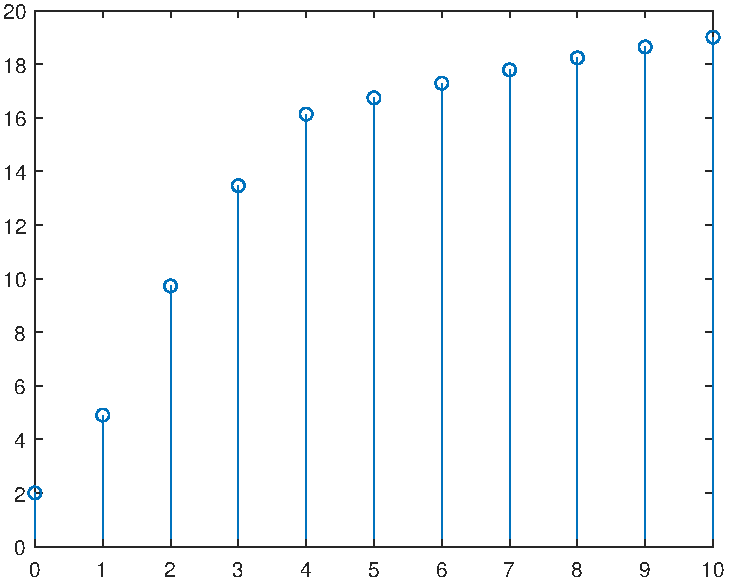
\includegraphics[width=1.8in]{problem1c.pdf}
    \end{center}
\end{figure}

\section*{Problem 2}

\paragraph{a)}

Let \(h[n]\) be the impulse response of the system. Then we have the following relationship.
\[y[n] = u[n]*h[n] = 0.5^nu[n]\]
Assume that \(h[n]\) is causal. Then if we evaluate both sides for given values of \(n=0,1,2,\ldots\) we obtain the following equations.
\begin{align*}
    1 &= h[0]\\
    \frac{1}{2} &= h[0] + h[1]\\
    \frac{1}{2^2} &= h[0] + h[1] + h[2]\\
    \frac{1}{2^3} &= h[0] + h[1] + h[2] + h[3]\\
    &\vdots
\end{align*}
Solving these yields the following function.
\[h[n] = -\frac{1}{2^n}u[n] + 2\delta[n]\]

\paragraph{b)}

This is true. Consider the system \(y[n]=x[n]*h[n]\) where \(x[n]\) and \(h[n]\) are both even.
Using the definition of convolution this system becomes the following.
\[y[n]=\sum_{k=-\infty}^\infty x[k]h[n-k]\]
We can show at \(-n\) this evaluates to the same value as at \(n\).
\begin{align*}
    y[-n] &= \sum_{k=-\infty}^\infty x[k]h[-n-k]\\
    &=\sum_{k=-\infty}^\infty x[-k]h[-n-k]\\
    &=\sum_{k^\prime=-\infty}^\infty x[k^\prime]h[-n+k^\prime]\\
    &=\sum_{k^\prime=-\infty}^\infty x[k^\prime]h[n-k^\prime]\\
    &=y[n]
\end{align*}
We were able to flip the signs of the indices for \(x[n]\) and \(h[n]\) since they are even, and
we used the substitution \(k^\prime=-k\). Thus since \(y[-n]=y[n]\) the output is even.

\section*{Problem 3}

\paragraph{a)}

By plugging in some values we can see that the output has the following behaviour.
\begin{align*}
    y[0] &= 0\\
    y[1] &= \frac{1}{2}\\
    y[2] &= \frac{3}{4}\\
    y[3] &= \frac{7}{8}\\
    &\vdots
\end{align*}
The following output equation fits this behaviour.
\[y[n] = \left(1-\frac{1}{2^n}\right)u[n-1]\]

\paragraph{b)}

By plugging in some values we can see that the output has the following behaviour.
\begin{align*}
    y[0] &= 1\\
    y[1] &= 1\\
    y[2] &= \frac{1}{2}\\
    y[3] &= \frac{1}{4}\\
    &\vdots
\end{align*}
The following output equation fits this behavior.
\[y[n] = u[-n] + \frac{1}{2^{n-1}}u[n-1]\]

\section*{Problem 4}

This function has a period of \(N=25\). Thus our fourier transform coefficients have the following form.
\[c_k=\frac{1}{25}\sum_{n=0}^{24}x[n] e^{-j\frac{2\pi k}{25}n}\]
We can rewrite our function as follows.
\begin{align*}
    x[n] &= 1+\cos(0.24\pi n)+3\sin(0.56\pi n)\\
    &=1+\frac{1}{2}e^{j\frac{6\pi}{25}n}+\frac{1}{2}e^{-j\frac{6\pi}{25}n}+\frac{3}{2j}e^{j\frac{14\pi}{25}n}-\frac{3}{2j}e^{-j\frac{14\pi}{25}n}\\
    &=1+\frac{1}{2}e^{j\frac{6\pi}{25}n}+\frac{3}{2j}e^{j\frac{14\pi}{25}n}-\frac{3}{2j}e^{j\frac{36\pi}{25}n}+\frac{1}{2}e^{j\frac{44\pi}{25}n}
\end{align*}
We were able to rewrite the terms with negative normalized frequencies by multiplying with \(1^n=e^{j2\pi n}\).
Thus the only coefficients that are not zero would be \(c_0\), \(c_3\), \(c_7\), \(c_{18}\), and \(c_{22}\), since
these values of \(k\) have a corresponding frequency component in \(x[n]\). We can select the correct
frequency components and calculate the coefficients as follows.
\begin{align*}
    c_0 &= \frac{1}{25}\sum_{n=0}^{24}1e^{-j\frac{2\pi \times 0}{25}n}\\
    &=\frac{1}{25}\sum_{n=0}^{24}1\\
    &=1
\end{align*}
Similar calculations yield the following coefficients.
\[c_0=1\qquad c_3=\frac{1}{2}\qquad c_7=\frac{3}{2j}\qquad c_{18}=-\frac{3}{2j}\qquad c_{22}=\frac{1}{2}\]
The magnitude and phase plots of the DTFS coefficients is shown below.
\begin{figure}[H]
    \begin{center}
        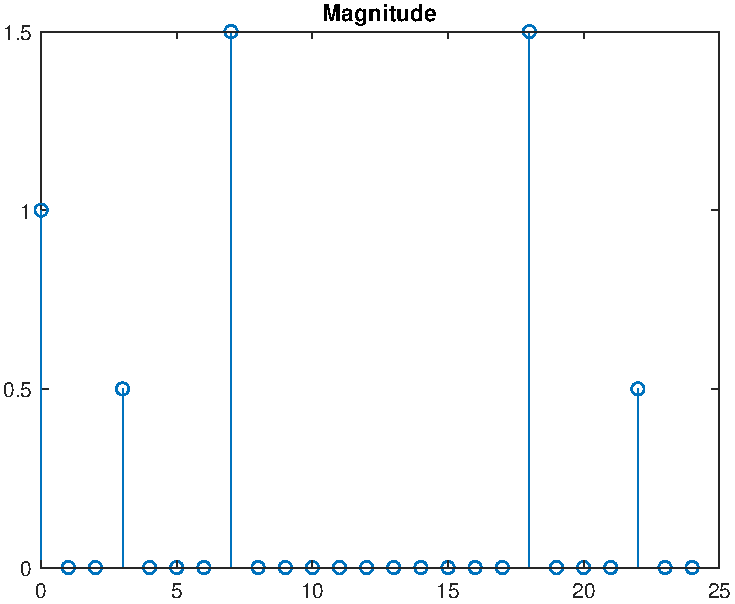
\includegraphics[width=2.5in]{problem4-mag.pdf}
        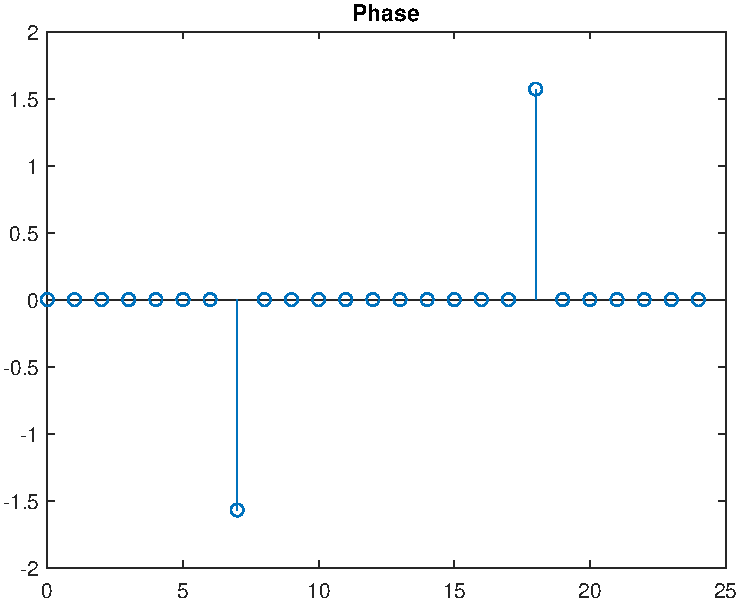
\includegraphics[width=2.5in]{problem4-phase.pdf}
    \end{center}
\end{figure}

\section*{Problem 5}

\paragraph{a)}

We will use the following definition for the DTFS coefficients.
\[\tilde{d}_k=\frac{1}{5}\sum_{n=0}^{4}\tilde{g}[n] e^{-j\frac{2\pi k}{5}n}\]
Then we have the following results.
\begin{align*}
    \tilde{d}_0&=\frac{1}{5}(4+1+2+3)=2\\
    \tilde{d}_1&=\frac{1}{5}\left(4+e^{-j\frac{4\pi}{5}}+2e^{-j\frac{6\pi}{5}}+3e^{-j\frac{8\pi}{5}}\right)=0.5+0.68819j\\
    \tilde{d}_2&=\frac{1}{5}\left(4+e^{-j\frac{8\pi}{5}}+2e^{-j\frac{12\pi}{5}}+3e^{-j\frac{16\pi}{5}}\right)=0.5+0.16246j\\
    \tilde{d}_3&=\frac{1}{5}\left(4+e^{-j\frac{12\pi}{5}}+2e^{-j\frac{18\pi}{5}}+3e^{-j\frac{24\pi}{5}}\right)=0.5-0.16246j\\
    \tilde{d}_4&=\frac{1}{5}\left(4+e^{-j\frac{16\pi}{5}}+2e^{-j\frac{24\pi}{5}}+3e^{-j\frac{32\pi}{5}}\right)=0.5-0.68819j
\end{align*}

\paragraph{b)}

We have that \(\tilde{g}[n]=\tilde{x}[n-1]\). Then we can apply the time shifting property as shown below.
\begin{align*}
    \tilde{d}_0&=e^{-j\frac{2\pi}{5}0}\tilde{c}_0=2\\
    \tilde{d}_1&=e^{-j\frac{2\pi}{5}1}\tilde{c}_0=0.5+0.68819j\\
    \tilde{d}_2&=e^{-j\frac{2\pi}{5}2}\tilde{c}_0=0.5+0.16243j\\
    \tilde{d}_3&=e^{-j\frac{2\pi}{5}3}\tilde{c}_0=0.5-0.16243j\\
    \tilde{d}_4&=e^{-j\frac{2\pi}{5}4}\tilde{c}_0=0.5-0.68819j
\end{align*}
This agrees with my previous results, except for rounding errors.

\end{document}